% Source PDF page 305 (printed p. 291)
\section{范数逼近}
\subsection{基本范数逼近问题}
最简单的范数逼近问题是如下形式的无约束问题：
\begin{equation}
\begin{array}{ll}\text{最小化}&\norm{Ax-b},\end{array}\tag{6.1}
\end{equation}
其中 $A\in\R^{m\times n}$ 和 $b\in\R^m$ 是问题数据，$x\in\R^n$ 是变量，$\norm{\cdot}$ 是 $\R^m$ 上的一个范数。范数逼近问题的解，有时称为 $Ax\approx b$ 在范数 $\norm{\cdot}$ 下的近似解。向量
\[r=Ax-b\]
称为该问题的\emph{残差}；它的各个分量有时称为与 $x$ 对应的单个残差。

范数逼近问题 (6.1) 是凸问题，而且总有解，即至少存在一个最优解。当且仅当 $b\in\mathcal R(A)$ 时，其最优值为零；不过，$b\notin\mathcal R(A)$ 时，这个问题才更有意思、更有用。不失一般性，可以假定 $A$ 的列线性无关；特别地，有 $m\ge n$。当 $m=n$ 时，最优点就是 $A^{-1}b$，因此可以假设 $m>n$。

\subsubsection*{逼近解释}
将 $Ax$ 写成
\[Ax=x_1a_1+\cdots+x_na_n,\]
其中 $a_1,\ldots,a_n\in\R^m$ 是 $A$ 的各列，便可看出：范数逼近问题的目标，是用 $A$ 的列的线性组合尽可能贴近地拟合或逼近向量 $b$，偏差则用范数 $\norm{\cdot}$ 衡量。

逼近问题也称为\emph{回归问题}。在这种表述下，向量 $a_1,\ldots,a_n$ 称为回归向量，而当 $x$ 是问题的最优解时，向量 $x_1a_1+\cdots+x_na_n$ 称为 $b$ 在这些回归向量上的回归。

% Source PDF page 306 (printed p. 292)
\subsubsection*{估计解释}
在根据不精确的线性向量测量来估计参数向量时，范数逼近问题有一种密切相关的解释。考虑线性测量模型
\[y=Ax+v,\]
其中 $y\in\R^m$ 是测量向量，$x\in\R^n$ 是待估计的参数向量，$v\in\R^m$ 是未知的测量误差，但假定其在范数 $\norm{\cdot}$ 下很小。估计问题是：给定 $y$，对 $x$ 作出合理猜测。

如果猜测 $x$ 的值是 $\widehat x$，实际上也就猜测 $v$ 的值为 $y-A\widehat x$。若认为较小的 $v$（按 $\norm{\cdot}$ 衡量）比较大的 $v$ 更可信，那么对 $x$ 最可信的猜测是
\[\widehat x=\argmin_z\norm{Az-y}.\]
（这些想法可以在统计框架下更正式地表述；见第7章。）

\subsubsection*{几何解释}
考虑子空间 $\mathcal A=\mathcal R(A)\subseteq\R^m$ 和点 $b\in\R^m$。点 $b$ 在范数 $\norm{\cdot}$ 下到子空间 $\mathcal A$ 的一个投影，是 $\mathcal A$ 中距 $b$ 最近的任意一点，即问题
\[\begin{array}{ll}\text{最小化}&\norm{u-b}\\\text{约束条件}&u\in\mathcal A\end{array}\]
的任意最优点。将 $\mathcal R(A)$ 的任意元素参数化为 $u=Ax$，可见求解范数逼近问题 (6.1)，等价于计算 $b$ 到 $\mathcal A$ 的一个投影。

\subsubsection*{设计解释}
范数逼近问题 (6.1) 也可以解释为一个最优设计问题。$n$ 个变量 $x_1,\ldots,x_n$ 是待确定取值的设计变量。向量 $y=Ax$ 给出 $m$ 个结果，假设它们是设计变量 $x$ 的线性函数。向量 $b$ 是目标结果或期望结果。我们希望选择一组设计变量，使其尽可能接近期望结果，即 $Ax\approx b$。残差向量 $r$ 可以解释为实际结果（即 $Ax$）与期望或目标结果（即 $b$）之间的偏差。如果用实际结果与期望结果之间的偏差范数衡量设计的好坏，那么范数逼近问题 (6.1) 就是寻找最佳设计的问题。

% Source PDF page 307 (printed p. 293)
\subsubsection*{加权范数逼近问题}
范数逼近问题的一个扩展是加权范数逼近问题
\[\text{最小化}\quad\norm{W(Ax-b)},\]
其中问题数据 $W\in\R^{m\times m}$ 称为加权矩阵。加权矩阵通常是对角矩阵，此时它对残差向量 $r=Ax-b$ 的不同分量赋予不同的相对权重。

加权范数问题可以看作采用范数 $\norm{\cdot}$、数据为 $\widetilde A=WA$、$\widetilde b=Wb$ 的范数逼近问题，因此可以按标准范数逼近问题 (6.1) 处理。另一种看法是，保留数据 $A$ 和 $b$，改用如下定义的 $W$ 加权范数：
\[\norm z_W=\norm{Wz}\]
（这里假定 $W$ 非奇异）。

\subsubsection*{最小二乘逼近}
最常见的范数逼近问题采用欧几里得范数，即 $\ell_2$ 范数。将目标函数平方，就得到一个等价问题，称为\emph{最小二乘逼近问题}：
\[\text{最小化}\quad\norm{Ax-b}_2^2=r_1^2+r_2^2+\cdots+r_m^2,\]
其目标是各个残差的平方和。将目标写成凸二次函数
\[f(x)=x^\T A^\T Ax-2b^\T Ax+b^\T b,\]
即可解析求解。当且仅当
\[\nabla f(x)=2A^\T Ax-2A^\T b=0,\]
点 $x$ 使 $f$ 最小；也就是说，当且仅当 $x$ 满足所谓的\emph{正规方程}
\[A^\T Ax=A^\T b.\]
正规方程总有解。由于假定 $A$ 的列线性无关，最小二乘逼近问题具有唯一解 $x=(A^\T A)^{-1}A^\T b$。

\subsubsection*{Chebyshev 逼近或极小极大逼近}
使用 $\ell_\infty$ 范数时，范数逼近问题
\[\text{最小化}\quad\norm{Ax-b}_\infty=\max\{|r_1|,\ldots,|r_m|\}\]
称为\emph{Chebyshev 逼近问题}或\emph{极小极大逼近问题}，因为它要最小化残差绝对值的最大值。Chebyshev 逼近问题可以写成线性规划
\[\begin{array}{ll}\text{最小化}&t\\\text{约束条件}&-t\one\preceq Ax-b\preceq t\one,\end{array}\]
变量为 $x\in\R^n$ 和 $t\in\R$。

% Source PDF page 308 (printed p. 294)
\subsubsection*{残差绝对值和逼近}
使用 $\ell_1$ 范数时，范数逼近问题
\[\text{最小化}\quad\norm{Ax-b}_1=|r_1|+\cdots+|r_m|\]
称为\emph{残差（绝对值）和逼近问题}；在估计问题中，也称为\emph{稳健估计}（原因很快就会清楚）。与 Chebyshev 逼近问题一样，$\ell_1$ 范数逼近问题可以写成线性规划
\[\begin{array}{ll}\text{最小化}&\one^\T t\\\text{约束条件}&-t\preceq Ax-b\preceq t,\end{array}\]
变量为 $x\in\R^n$ 和 $t\in\R^m$。

\subsection{惩罚函数逼近}
在 $1\le p<\infty$ 的 $\ell_p$ 范数逼近中，目标为
\[(|r_1|^p+\cdots+|r_m|^p)^{1/p}.\]
如同最小二乘问题，可以考虑目标函数为
\[|r_1|^p+\cdots+|r_m|^p\]
的等价问题。这个目标是残差的可分离对称函数。特别地，目标仅取决于残差的幅度分布，也就是排序后的残差。

我们将研究 $\ell_p$ 范数逼近问题的一种有用推广，其目标同样只取决于残差的幅度分布。\emph{惩罚函数逼近问题}的形式为
\begin{equation}
\begin{array}{ll}\text{最小化}&\phi(r_1)+\cdots+\phi(r_m)\\\text{约束条件}&r=Ax-b,\end{array}\tag{6.2}
\end{equation}
其中 $\phi:\R\to\R$ 称为（残差）惩罚函数。假定 $\phi$ 为凸函数，那么惩罚函数逼近问题就是凸优化问题。在许多情况下，惩罚函数 $\phi$ 还是对称的、非负的，并满足 $\phi(0)=0$，不过分析中不使用这些性质。

\subsubsection*{解释}
惩罚函数逼近问题 (6.2) 可以作如下解释。选定 $x$ 后，就得到对 $b$ 的逼近 $Ax$，以及对应的残差向量 $r$。惩罚函数对残差的每个分量赋予代价或惩罚 $\phi(r_i)$；总惩罚是所有单个残差惩罚之和，即 $\phi(r_1)+\cdots+\phi(r_m)$。不同的 $x$ 会产生不同残差，从而带来不同的总惩罚。惩罚函数逼近问题要使残差造成的总惩罚最小。

% Source PDF page 309 (printed p. 295)
\begin{figure}[htbp]\centering
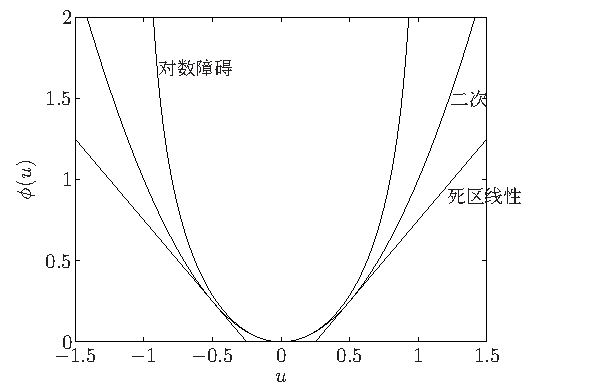
\includegraphics[width=.65\textwidth]{ch06-01.pdf}
\caption*{图6.1\quad 几种常用惩罚函数：二次惩罚函数 $\phi(u)=u^2$、死区宽度为 $a=1/4$ 的死区线性惩罚函数，以及限制值为 $a=1$ 的对数障碍惩罚函数。}
\end{figure}
\begin{origexample}{6.1}
几种常用惩罚函数及其对应的逼近问题。
\begin{itemize}
\item 取 $\phi(u)=|u|^p$，其中 $p\ge1$，惩罚函数逼近问题就等价于 $\ell_p$ 范数逼近问题。特别地，二次惩罚函数 $\phi(u)=u^2$ 给出最小二乘逼近或欧几里得范数逼近；绝对值惩罚函数 $\phi(u)=|u|$ 给出 $\ell_1$ 范数逼近。
\item 死区线性惩罚函数（死区宽度 $a>0$）为
\[\phi(u)=\begin{cases}0,&|u|\le a,\\|u|-a,&|u|>a.\end{cases}\]
对于小于 $a$ 的残差，死区线性函数不施加惩罚。
\item 对数障碍惩罚函数（限制值 $a>0$）为
\[\phi(u)=\begin{cases}-a^2\log\bigl(1-(u/a)^2\bigr),&|u|<a,\\\infty,&|u|\ge a.\end{cases}\]
对于大于 $a$ 的残差，对数障碍惩罚函数施加无穷大的惩罚。
\end{itemize}
图6.1绘出了死区线性、对数障碍和二次惩罚函数。注意，当 $|u/a|\le0.25$ 时，对数障碍函数与二次惩罚非常接近（见习题6.1）。
\end{origexample}

将惩罚函数乘以一个正数，不影响惩罚函数逼近问题的解，因为这只相当于将目标函数作同样缩放。但惩罚函数的形状，会极大地影响惩罚函数逼近问题的解。

% Source PDF page 310 (printed p. 296)
粗略地说，$\phi(u)$ 衡量我们对取值为 $u$ 的残差有多不满意。如果 $u$ 很小时 $\phi(u)$ 也很小（甚至为零），就表示我们对这些取值的残差不太在意（或完全不在意）。如果 $\phi(u)$ 随 $u$ 增大而迅速增长，就表示我们很不希望出现大残差；如果 $\phi$ 在某个区间外取无穷大，则表示该区间之外的残差不可接受。这一简单解释，既有助于理解惩罚函数逼近问题的解，也为选择惩罚函数提供了指引。

例如，比较 $\ell_1$ 范数逼近和 $\ell_2$ 范数逼近，它们的惩罚函数分别为 $\phi_1(u)=|u|$ 和 $\phi_2(u)=u^2$。当 $|u|=1$ 时，两者赋予相同惩罚。对于较小的 $u$，有 $\phi_1(u)\gg\phi_2(u)$，因此与 $\ell_2$ 范数逼近相比，$\ell_1$ 范数逼近对小残差赋予更大的相对权重。对于较大的 $u$，有 $\phi_2(u)\gg\phi_1(u)$，所以 $\ell_1$ 范数逼近对大残差赋予的权重小于 $\ell_2$ 范数逼近。对大、小残差的相对权重不同，会反映在相应逼近问题的解中：与 $\ell_2$ 范数逼近解相比，$\ell_1$ 范数逼近问题的最优残差幅度分布往往包含更多为零或很小的残差。相反，$\ell_2$ 范数解中较大的残差通常相对较少，因为大残差在 $\ell_2$ 范数逼近中的惩罚远大于在 $\ell_1$ 范数逼近中的惩罚。

\subsubsection*{一个例子}
下面用一个例子说明这些想法。取矩阵 $A\in\R^{100\times30}$ 和向量 $b\in\R^{100}$（随机选取，但结果具有代表性），计算 $Ax\approx b$ 的 $\ell_1$、$\ell_2$ 范数近似解，以及采用死区线性惩罚（$a=0.5$）和对数障碍惩罚（$a=1$）的惩罚函数逼近解。图6.2给出了这四种惩罚函数，以及这四种惩罚逼近所对应的最优残差幅度分布。从惩罚函数图可以看出：
\begin{itemize}
\item $\ell_1$ 范数惩罚对小残差赋予的权重最大，对大残差赋予的权重最小。
\item $\ell_2$ 范数惩罚对小残差的权重很小，但对大残差的权重很大。
\item 死区线性惩罚函数不惩罚小于 $0.5$ 的残差，而对大残差也只赋予相对较小的权重。
\item 对数障碍惩罚对小残差的权重与 $\ell_2$ 范数惩罚很接近，但对大于约 $0.8$ 的残差赋予很大权重，对大于 $1$ 的残差则赋予无穷大权重。
\end{itemize}
从幅度分布中可以清楚地看到以下几点：
\begin{itemize}
\item 对 $\ell_1$ 最优解，很多残差为零或非常小；同时它也包含相对更多的大残差。
\end{itemize}

% Source PDF page 311 (printed p. 297)
\begin{figure}[htbp]\centering
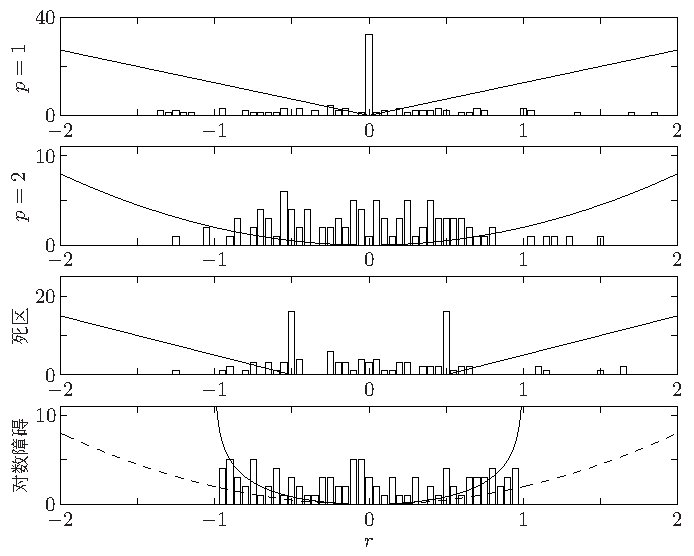
\includegraphics[width=.78\textwidth]{ch06-02.pdf}
\caption*{图6.2\quad 四种惩罚函数对应的残差幅度直方图；图中也绘出了经缩放的惩罚函数以供参考。对数障碍图中还以虚线绘出了二次惩罚函数。}
\end{figure}

% Source PDF page 312 (printed p. 298)
\begin{figure}[htbp]\centering
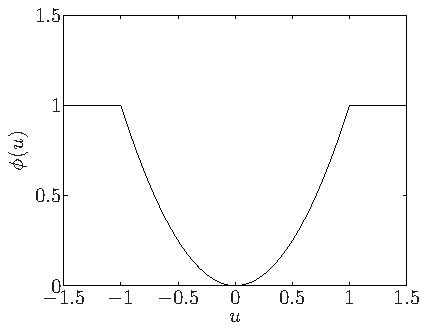
\includegraphics[width=.58\textwidth]{ch06-03.pdf}
\caption*{图6.3\quad 对超过阈值（本例中为 $1$）的残差施加固定惩罚的非凸惩罚函数：当 $|u|\le1$ 时，$\phi(u)=u^2$；当 $|u|>1$ 时，$\phi(u)=1$。因此，用该函数进行惩罚逼近对离群值相对不敏感。}
\end{figure}
\begin{itemize}
\item $\ell_2$ 范数逼近有许多中等大小的残差，而较大的残差相对较少。
\item 对死区线性惩罚，可以看到许多残差的值为 $\pm0.5$，恰好落在不受惩罚的“免费”区域边缘。
\item 对对数障碍惩罚，没有残差的幅度大于 $1$；除此之外，其残差分布与 $\ell_2$ 范数逼近的残差分布相似。
\end{itemize}

\subsubsection*{对离群值或大误差的敏感性}
在估计或回归问题中，\emph{离群值}是噪声 $v_i$ 相对较大的测量值 $y_i=a_i^\T x+v_i$。它常与错误数据或有缺陷的测量有关。存在离群值时，对 $x$ 的任何估计所对应的残差向量中，都会有一些较大的分量。理想情况下，希望能判断哪些测量是离群值，把它们从估计过程中剔除，或者大幅降低它们在估计中的权重。（不过，不能对很大的残差赋予零惩罚，否则最优点很可能会使所有残差都很大，从而使总惩罚为零。）可以使用惩罚函数逼近，并采用如下惩罚函数来实现这一想法：
\begin{equation}
\phi(u)=\begin{cases}u^2,&|u|\le M,\\M^2,&|u|>M,\end{cases}\tag{6.3}
\end{equation}
如图6.3所示。对于小于 $M$ 的残差，该惩罚函数与最小二乘一致；但对大于 $M$ 的残差，无论究竟大多少，都施加固定惩罚。也就是说，超过 $M$ 的残差被忽略，假定它们来自离群值或错误数据。遗憾的是，惩罚函数 (6.3) 非凸，相应的惩罚函数逼近问题会变成困难的组合优化问题。

% Source PDF page 313 (printed p. 299)
\begin{figure}[htbp]\centering
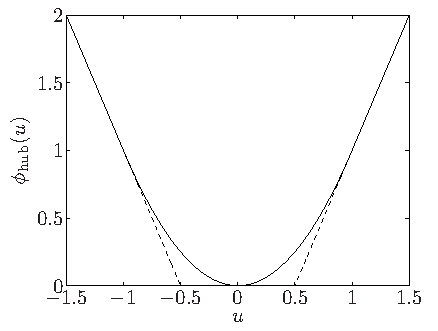
\includegraphics[width=.58\textwidth]{ch06-04.pdf}
\caption*{图6.4\quad 实线是取 $M=1$ 的稳健最小二乘惩罚函数，即 Huber 惩罚函数 $\phi_{\rm hub}$。当 $|u|\le M$ 时它是二次的，当 $|u|>M$ 时呈线性增长。}
\end{figure}
基于惩罚函数的估计方法对离群值的敏感程度，取决于惩罚函数对大残差所赋予的相对惩罚。如果只考虑会产生凸优化问题的凸惩罚函数，那么对离群值最不敏感的，是在 $u$ 较大时像 $|u|$ 那样线性增长的 $\phi(u)$。具有这一性质的惩罚函数有时称为\emph{稳健}的，因为相应的惩罚函数逼近方法对离群值或大误差的敏感性，比最小二乘等方法低得多。

一个显然的稳健惩罚函数是 $\phi(u)=|u|$，它对应 $\ell_1$ 范数逼近。另一个例子是\emph{稳健最小二乘}惩罚函数，即 \emph{Huber 惩罚函数}：
\begin{equation}
\phi_{\rm hub}(u)=\begin{cases}u^2,&|u|\le M,\\M(2|u|-M),&|u|>M,\end{cases}\tag{6.4}
\end{equation}
如图6.4所示。对于小于 $M$ 的残差，该惩罚函数与最小二乘惩罚函数一致；对较大的残差，则转为类似 $\ell_1$ 范数的线性增长。Huber 惩罚函数可以在下述意义下看作离群惩罚函数 (6.3) 的凸近似：当 $|u|\le M$ 时，两者相同；当 $|u|>M$ 时，Huber 惩罚函数是与离群惩罚函数 (6.3) 最接近的凸函数。

\begin{origexample}{6.2}
\emph{稳健回归。}图6.5给出了平面上的42个点 $(t_i,y_i)$，其中有两个明显的离群值（一个在左上方，另一个在右下方）。虚线是用直线 $f(t)=\alpha+\beta t$ 对这些点作最小二乘逼近的结果。系数 $\alpha$、$\beta$ 由下述最小二乘问题得到：
\[\text{最小化}\quad\sum_{i=1}^{42}(y_i-\alpha-\beta t_i)^2,\]
变量为 $\alpha$ 和 $\beta$。最小二乘逼近直线明显偏离了这些点主要分布的方向，转向了两个离群值。

% Source PDF page 314 (printed p. 300)
\begin{figure}[htbp]\centering
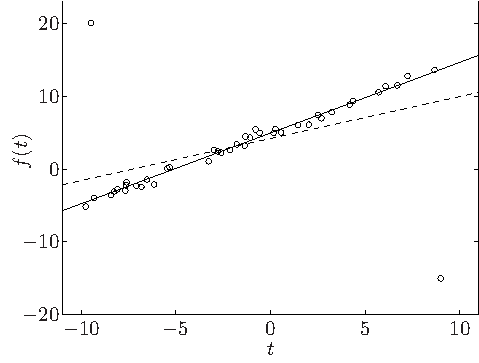
\includegraphics[width=.62\textwidth]{ch06-05.pdf}
\caption*{图6.5\quad 图中的42个圆圈表示可由仿射函数很好逼近的点，但左上方和右下方两个离群值例外。虚线是直线 $f(t)=\alpha+\beta t$ 的最小二乘拟合，它偏离了点的主要分布方向，转向离群值。实线是最小化 $M=1$ 的 Huber 惩罚函数所得到的稳健最小二乘拟合；它对非离群数据的拟合好得多。}
\end{figure}
实线是最小化 Huber 惩罚函数
\[\text{最小化}\quad\sum_{i=1}^{42}\phi_{\rm hub}(y_i-\alpha-\beta t_i),\]
所得到的稳健最小二乘逼近，其中 $M=1$。这个逼近受离群值的影响小得多。
\end{origexample}

由于 $\ell_1$ 范数逼近是各种凸惩罚函数逼近方法中对离群值最稳健的方法之一，它有时称为\emph{稳健估计}或\emph{稳健回归}。$\ell_1$ 范数估计的稳健性也可以从统计框架理解；见第353页。

\subsubsection*{小残差与 $\ell_1$ 范数逼近}
也可以把注意力放在小残差上。最小二乘逼近对小残差赋予的权重很小，因为当 $u$ 很小时，$\phi(u)=u^2$ 非常小。死区线性惩罚函数等对小残差的惩罚为零。对于在残差较小时取值非常小的惩罚函数，可以预期最优残差会比较小，但不会非常小。粗略地说，把一个已经很小的残差继续缩小，几乎或完全没有收益。

相反，$\phi(u)=|u|$ 这类对小残差赋予较大相对权重的惩罚函数，对应于 $\ell_1$ 范数逼近，往往会产生大量非常小、甚至恰好为零的最优残差。这意味着，在 $\ell_1$ 范数逼近中，通常会发现许多方程被精确满足，即对许多 $i$ 有 $a_i^\T x=b_i$。这一现象可以从图6.2看到。
